\documentclass{article}

% Language setting
% Replace `english' with e.g. `spanish' to change the document language
\usepackage[english]{babel}
\usepackage{indentfirst}
% Set page size and margins
% Replace `letterpaper' with `a4paper' for UK/EU standard size
\usepackage[letterpaper,top=2cm,bottom=2cm,left=3cm,right=3cm,marginparwidth=1.75cm]{geometry}

% Useful packages
\usepackage{amsmath}
\usepackage{graphicx}
\usepackage[colorlinks=true, allcolors=blue]{hyperref}

\title{A 40Gbps Economic Extension Board and FPGA-based Testing Platform}
\author{Te-Hui Chen, Student Member, IEEE\\David C. Keezer, Fellow, IEEE}
\date{October 25, 2016}
\begin{document}
\maketitle

\begin{abstract}
This paper describes a low-cost extension board used together with an FPGA-based test platform that enables digital testing up to 40Gbps. The high bandwidth of the board allows testing performance needed for future high-speed standards. An FPGA main board is built to control this plugin board for testing across a wide range of data-rates. The FPGA itself supports to transmit and receive signals up to 10Gbps. This economic plugin test module is used to multiplex four high-speed channels from the FPGA into a single 40Gbps serial bit stream. 
\end{abstract}

\section{Introduction}
Traditionally automated test equipment (ATE) has played a critical role of testing the most advanced high-speed electronic designs. However, the high cost and constraints of conventional ATE has been mostly limited to several Gbps applications. This data rate is not sufficient for the most advanced designs today. There are several methods to deal with this issue. ATE extensions\cite{bib1} provide the ability of multi-channel and high speed testing. However, the price and the power consumption are still high. Built-In Self-Test (BIST)\cite{bib2} is another way to test high-speed digital systems. In this scheme, BIST uses several low-speed signals from an ATE and generates high-speed data for digital testing within the device-under-test (DUT). This design can be built inside a DUT module and may also extend the use of older ATE. The draw-back of custom BIST is that it may have limited flexibility to handle a variety of IO standards. In other words, a new test system design is needed if a new 
standard comes into the market. To replace those powerful but expensive ATEs, FPGAs are a popular solution\cite{bib3}3 to be applied to low-cost electronic test. 

\section{FPGA-BASED TESTING PLATFORM DESIGN}
The FPGA-based testing platform is implemented using a 28nm Xilinx Kintex-7 FPGA, which supports up to 16 high speed channels, 500 moderate-speed I/Os, and millions of logic cells for implementing various testing algorithms. The FPGA here plays the similar role of the ATE core system, which performs different testing strategies for different applications of DUTs. A block diagram of this testing main board is shown in Fig.\ref{fig:fig1}. The core control center is the FPGA, with auxiliary controls such as USB and SPI. The I/Os of the FPGA are connected to four high-speed multi-pin connectors. Those connectors, with higher than 10GHz bandwidth per signal, each carry up to 10Gbps between the FPGA and the plugin modules. Each connector has 100 pins. Therefore it will support the four 10Gbps speed channels (16 lanes total for differential and dual
\par
Although the performance of FPGA itself is sufficient for most applications, there are still some testing features that cannot be obtained within the FPGA. Therefore on this platform, four extension slots are reserved to add these features and extend the function of the FPGA. The 40Gbps extension board utilizes the FPGA high-speed I/O channels and moderate speed I/Os that connect to those extension slots to implement the anticipated new testing strategies.
\begin{figure}
\centering
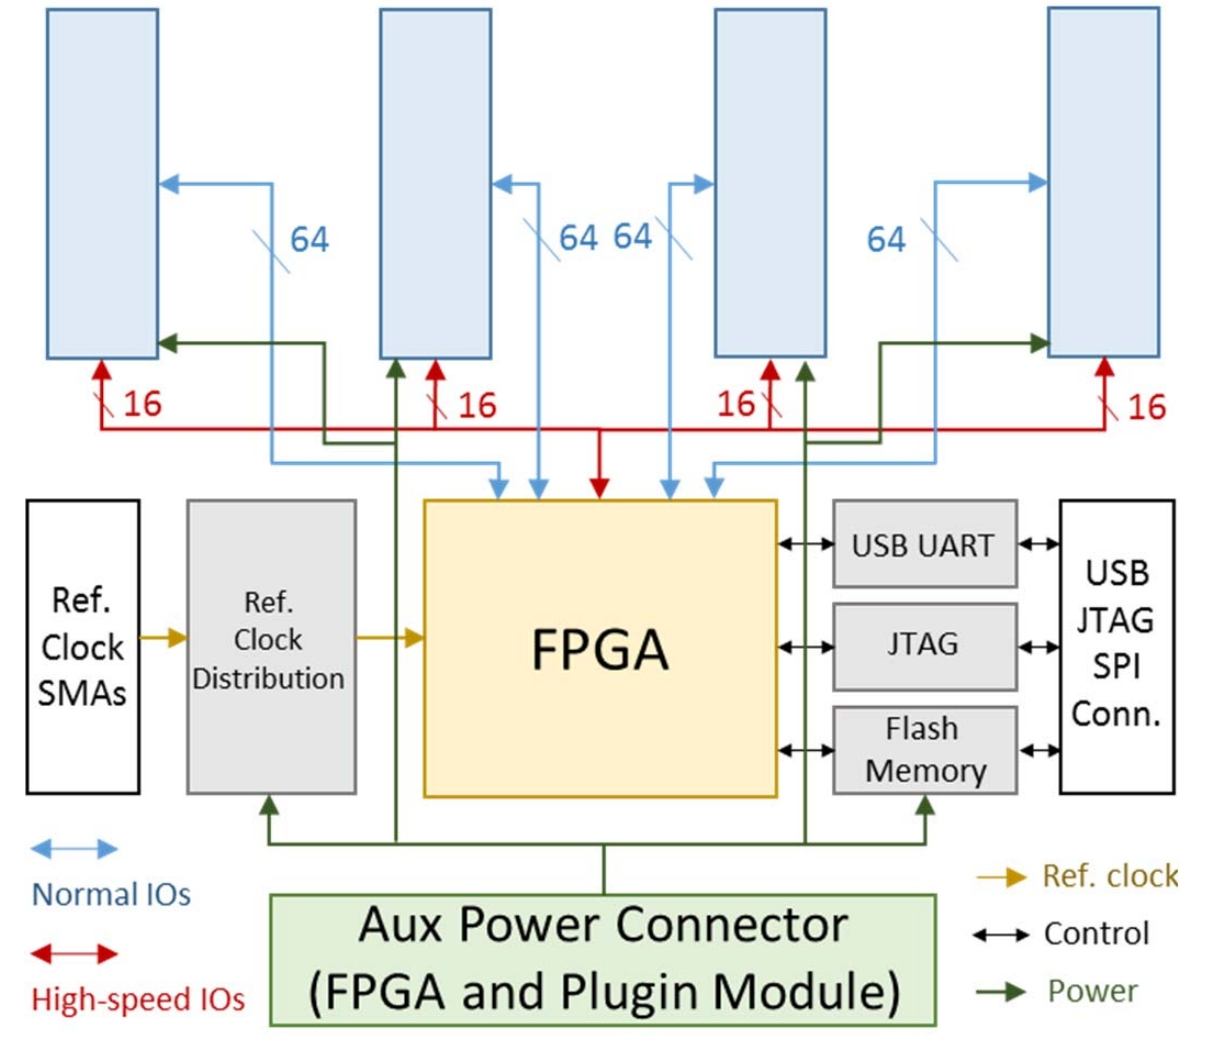
\includegraphics[width=0.5\textwidth]{fig1.png}
\caption{\label{fig:fig1}FPGA-based testing platform.}
\end{figure}

\section{40GBPS TRASMISSION BOARD DESIGN}
The basic concept to perform 40Gbps transmission is to build an extension module to plugin into the main board and extend the function of the FPGA. The simplified operation can be described as follows: In the transmitter side, the extension board takes four 10Gbps high-speed signals from the FPGA main board, and multiplexes (MUXes) those signals to form a 40Gbps serial signal. On the receiver side, we connect the DUT high speed signal back to a 40Gbps receiver/deserializer to obtain four 10Gbps signals so that the FPGA is able to receive the data in 4-bit parallel words. Fig.\ref{fig:fig2} shows the architecture of this extension board. The blue arrows show the signal direction of transmission. The FPGA main board generates PRBS or user defined data patterns and serializes this data to create 10Gbps signals. The high-performance connectors bring four-channel differential 10Gbps GTX signals from FPGA main board to this module. These differential signals go into a high-speed HMC847 MUX/serializer chip. The MUX chip uses a 20GHz delayed reference clock provided by an HMC910 delay chip to serialize the four 10Gbps signals to obtain a 40Gbps signal. The HMC910 delay chip takes the reference clock from an E8257D signal generator and adds a programmed delay up to maximum 70ps. The delay chip allows us to control the sampling phase of the serializer, which is critical for synthesizing the high-speed signal, and defines the phase of the 40 Gbps test signal. 

\begin{figure}
\centering
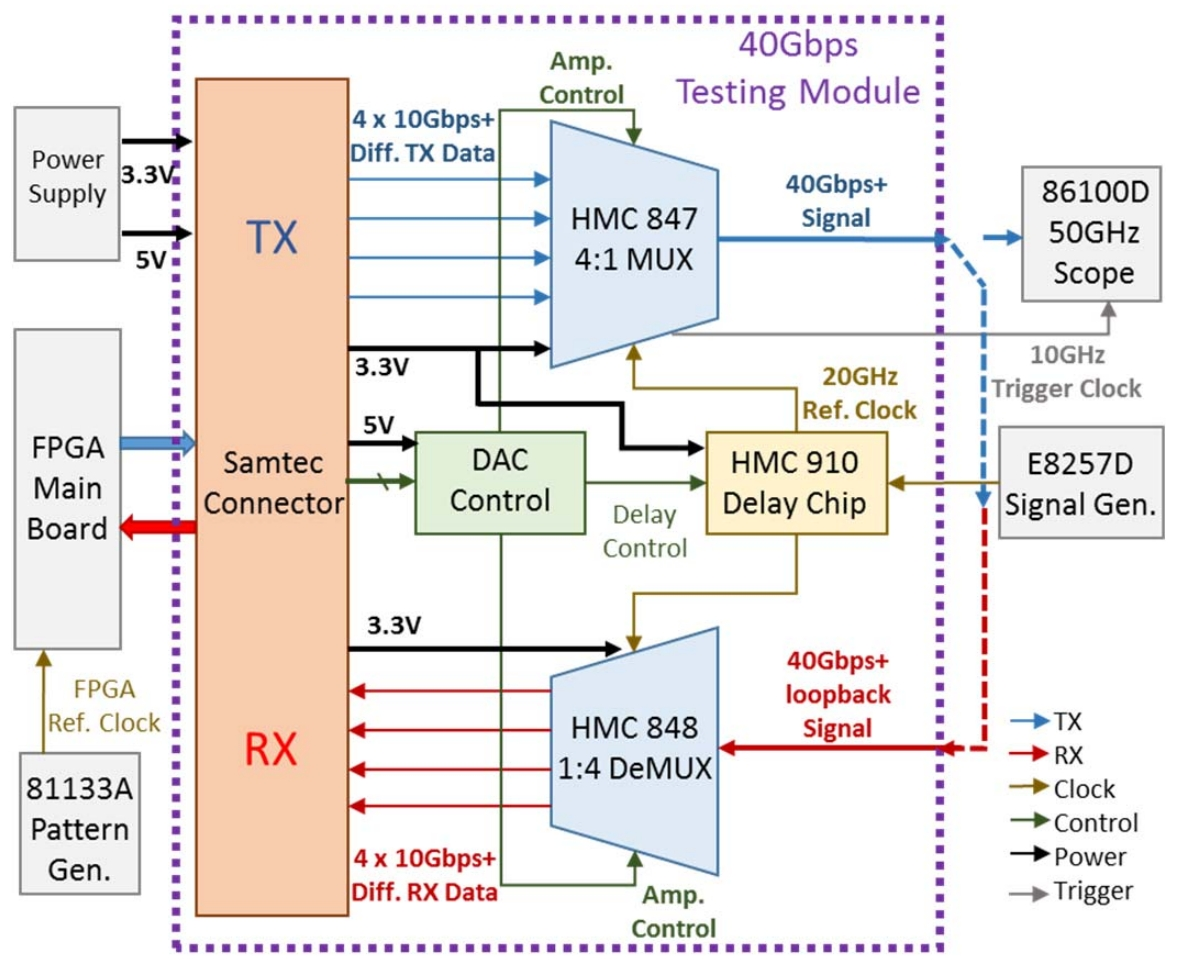
\includegraphics[width=0.5\textwidth]{fig2.png}
\caption{\label{fig:fig2}40Gbps extension board logic diagram.}
\end{figure}


\section{MEASUREMENTS AND RESULTS}
This section demonstrates the performance of the 40Gbps extension board. The measurements use a Keysight 86100D O-scope with a 54752A 50GHz sampling module. The scope is triggered by a divided-by-two clock from the HMC847. The sampling clock is generated by a Keysight E8257D 40GHz signal generator. The signal in the following figures is AC coupled, and is measured differentially. In Fig.\ref{fig:fig3}, the FPGA is programmed to output four channels of 10Gbps signals and the sampling clock is set to run at 20GHz to get 40Gbps data output. The jitter is as low at 1.5ps RMS (12ps total), and the rising and falling times are around 15ps. The amplitude of the signal is adjusted by a voltage control pin on the board from a DAC. Considering the random jitter of the O-scope trigger circuit is about 1ps RMS, and the jitter added in the data transmission (effect of cable, connectors, and PCB), the jitter performance is about as expected. Fig.\ref{fig:fig4} shows the example of the extension board output at 40Gbps with larger amplitudes at 650mV differential peak to peak. The small signal (200mV) in Fig.3 is close to the minimum specified for the MUX part. The data eyes are still open and usable even at this full-rate of 40Gbps. The rising/fall time for larger amplitude signals increases to about 18ps. The jitter at this frequency was found to be about 12ps over the amplitude range.

\begin{figure}
\centering
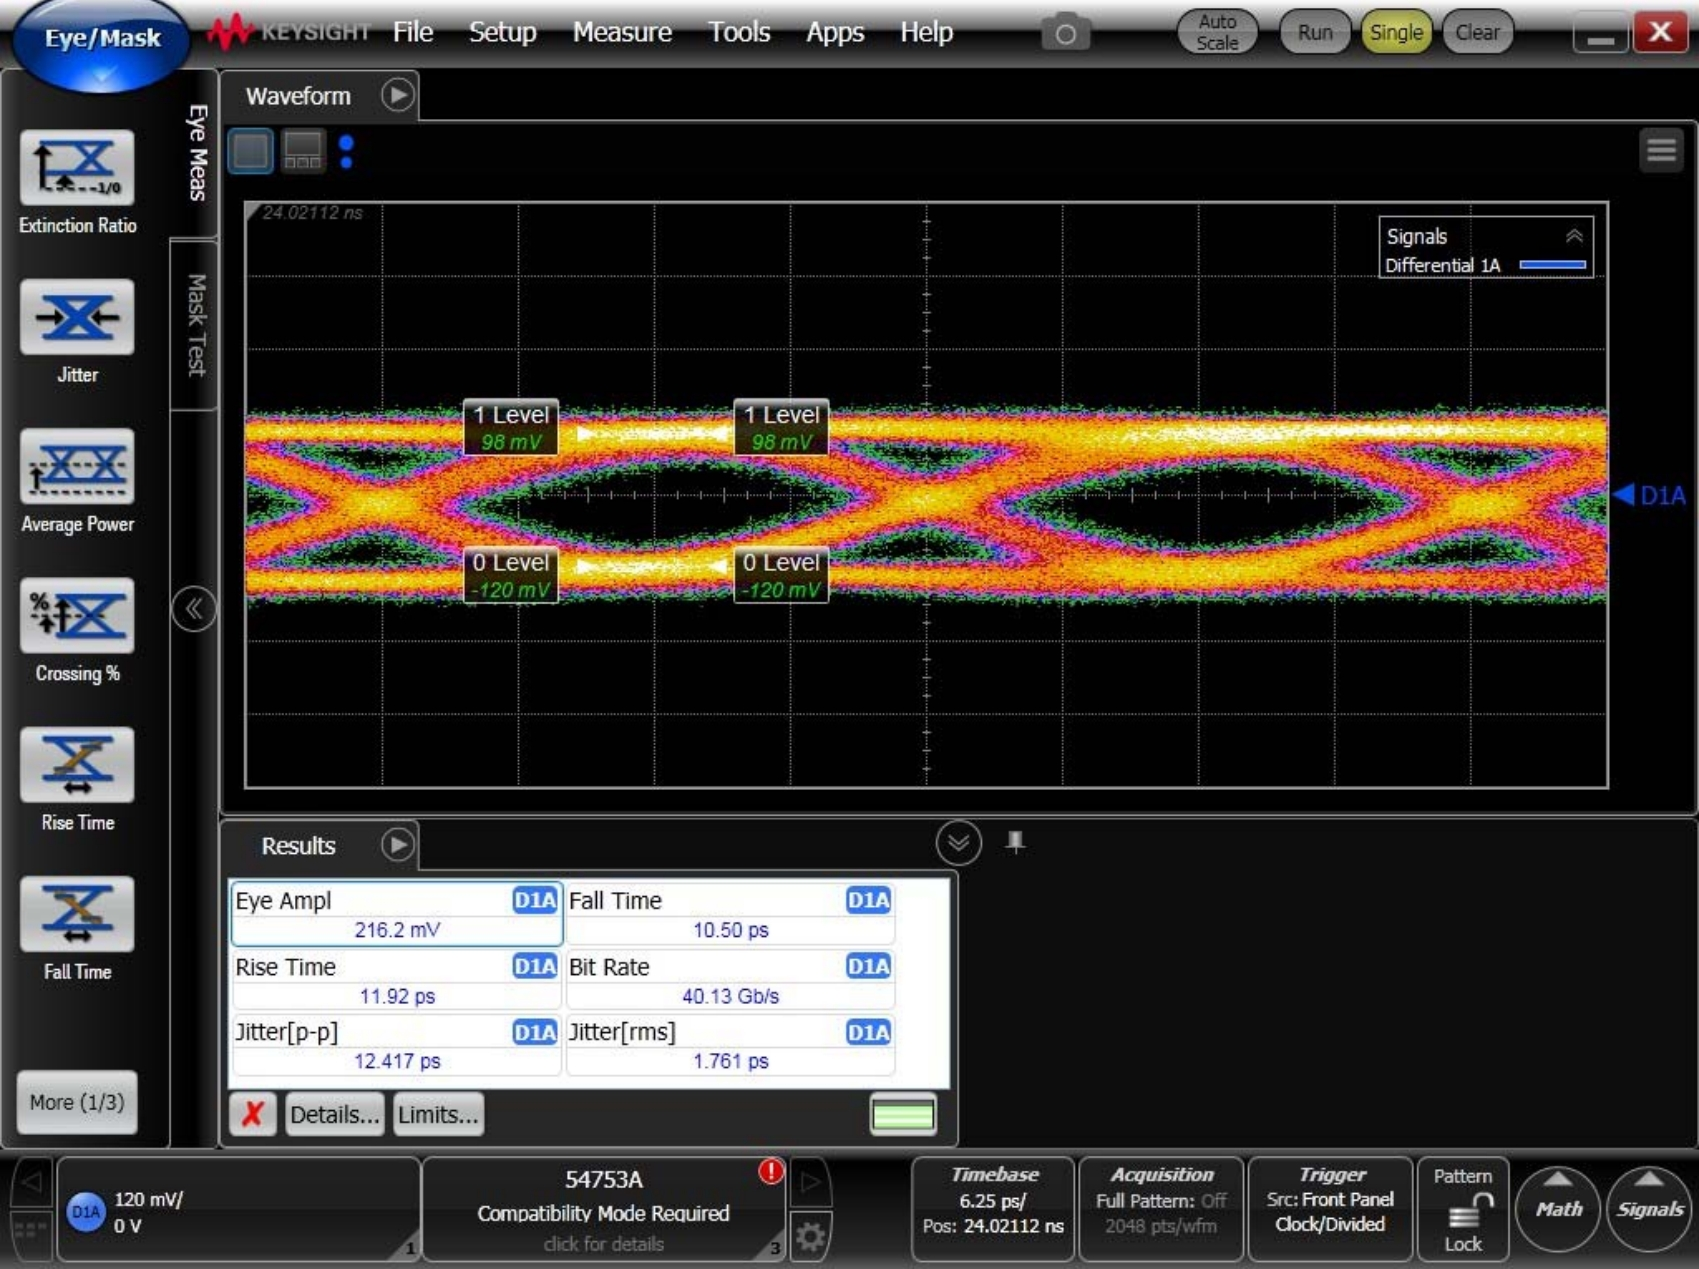
\includegraphics[width=0.5\textwidth]{fig3.png}
\caption{\label{fig:fig3}Extension board output with PRBS-31 pattern at 40Gbps(200mV).}
\end{figure}

\begin{figure}
\centering
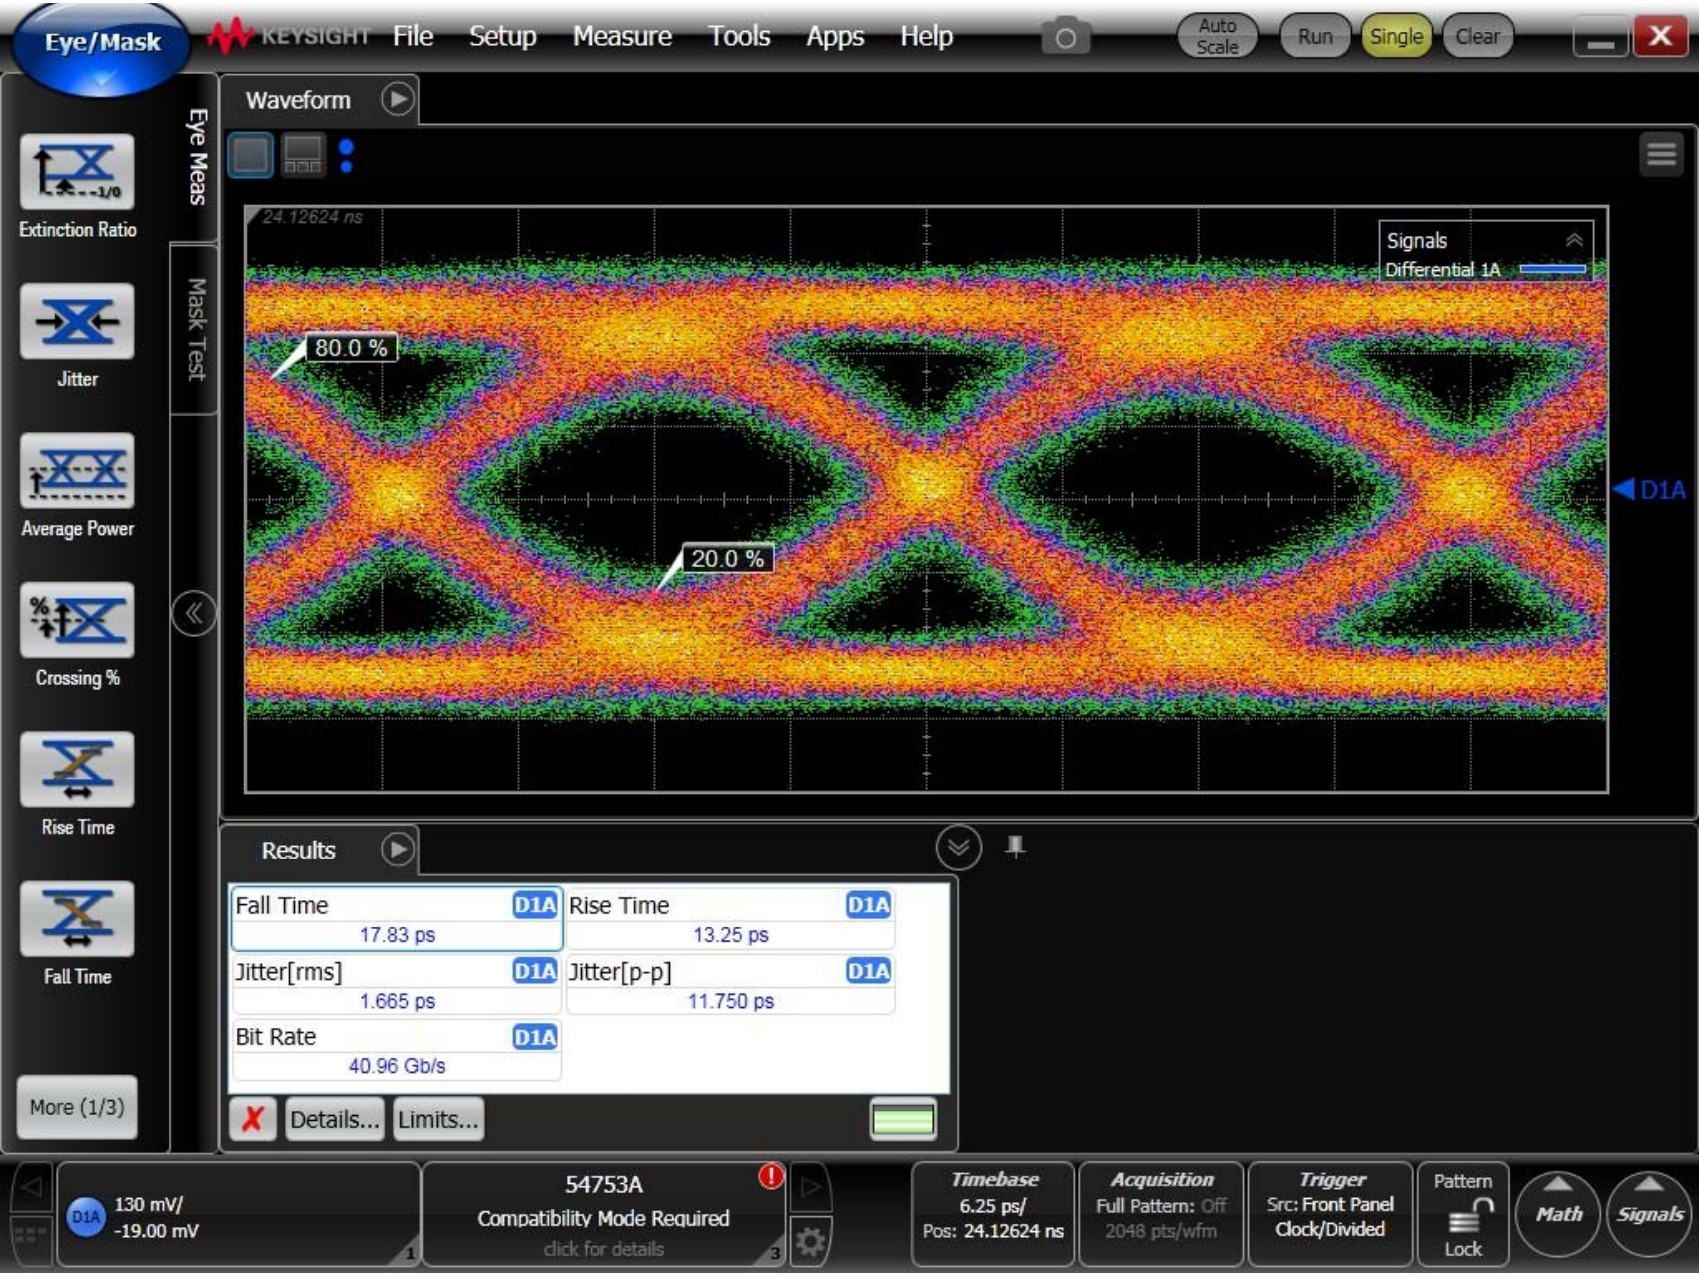
\includegraphics[width=0.5\textwidth]{fig4.png}
\caption{\label{fig:fig4}Extension board transmission at 40Gbps with 650mV amplitude.(6.25ps/div, 130mV/div) }
\end{figure}

\section{CONCLUSIONS}
This paper presented a low cost extension board which is implemented to extend FPGA output data rates up to 40Gbps. With this module board plugin, the testing platform is able to extend typical FPGA outputs (~10Gbps) to operate at very high data rates (up to 40 Gbps) with 15ps rising/fall times and about 12ps jitter. The amplitude, phase delay, and duty cycle are controllable, which enables characterization and go/no-Go testing across a wide range of I/O signaling standards in the future. 



\bibliographystyle{plain}
\bibliography{sample}

\end{document}
